\documentclass[12pt]{article}
\topmargin= -0.4in
\textheight = +8.9in
\oddsidemargin = 0.05in
\evensidemargin = 0.05in
\textwidth = 6.5in
\usepackage{times}
%\usepackage{babel}
\usepackage{graphicx}
\usepackage[T1]{fontenc}
\usepackage{lmodern}
\usepackage{amssymb,amsmath}
\usepackage{ifxetex,ifluatex}
\usepackage{fixltx2e} % provides \textsubscript
% use upquote if available, for straight quotes in verbatim environments
\IfFileExists{upquote.sty}{\usepackage{upquote}}{}
\ifnum 0\ifxetex 1\fi\ifluatex 1\fi=0 % if pdftex
  \usepackage[utf8]{inputenc}
\else % if luatex or xelatex
  \ifxetex
    \usepackage{mathspec}
    \usepackage{xltxtra,xunicode}
  \else
    \usepackage{fontspec}
  \fi
  \defaultfontfeatures{Mapping=tex-text,Scale=MatchLowercase}
  \newcommand{\euro}{€}
\fi
% use microtype if available
\IfFileExists{microtype.sty}{\usepackage{microtype}}{}
\usepackage{longtable,booktabs}
\ifxetex
  \usepackage[setpagesize=false, % page size defined by xetex
              unicode=false, % unicode breaks when used with xetex
              xetex]{hyperref}
\else
  \usepackage[unicode=true]{hyperref}
\fi
\hypersetup{breaklinks=true,
            bookmarks=true,
            pdfauthor={},
            pdftitle={},
            colorlinks=true,
            citecolor=blue,
            urlcolor=blue,
            linkcolor=black,
            pdfborder={0 0 0}}
\urlstyle{same}  % don't use monospace font for urls
\setlength{\parindent}{0pt}
\setlength{\parskip}{6pt plus 2pt minus 1pt}
\setlength{\emergencystretch}{3em}  % prevent overfull lines
\setcounter{secnumdepth}{0}

\begin{document}

\noindent
\thispagestyle{empty}
\underline{\bf Master's Paper of the Department of Statistics, the
  University of Chicago} 
\\~~(Internal document only, not for circulation) 

\vspace{1.8in}
\begin{center}
{\bf\LARGE Hidden Structure of Text Data } \\~\\
{Latent Topic Models and Sentiment Analysis}
\\~\\
%{\bf\Large --- A Sample Format}


\vspace{1.4in}
{\Large Nelson Auner}

\vspace{1.3in}
{\Large Advisors: Prof. Matt Taddy, Prof. Steven Stigler \\{\small }}

\end{center}

\vspace{.6in}
{\Large Approved} ~\underline{~~~~~~~~~~~~~~~~~~~~~~~~~~~~~~~~~~~~~~~~~~~~~~
~~~~~~~~~~~~~~~~~~~~~~~~~~~~~~~~~}

\vspace{.2in}
{\Large Date} ~\underline{~~~~~~~~~~~~~~~~~~~~~~~~~~~~~~~~~~~~~~~~~~~~~~~~~~~~
~~~~~~~~~~~~~~~~~~~~~~~~~~~~~~~~~~~}


\newpage
\pagestyle{plain}
\setcounter{page}{1}

\begin{abstract}

\vspace{7mm}\noindent 

This paper introduces a variant to existing models of multinomial
regression for text analysis. Using the base model introduced by Taddy
(2013), we extend the data-generating model to incorporate topics not
explained by existing Metadata. In doing so, we seek to both increase
the prediction accuracy over existing techniques, bridge the gap between
multinomial regression and standard topic models, and investigate
methods for discovering new topics in a corpus. We explore computational
aspects of our approach, provide software for parallelization of the
algorithm, and conclude by proposing areas of future research.

\end{abstract}

%\newpage
\vspace{1.5in}
\tableofcontents


\newpage


\section{Introduction}

\subsection{Text Data}



%
\includegraphics{chick}

Multinomial models are a common way of modeling annotated text.
Typically, text information is naturally grouped by documents, and each
document is represented by counts of words, or "tokens". A document might be a
single written text (e.g.~an academic article), or a collection of works
by the same author (e.g.~all of the lyrics of an album by the rolling
stones) A token is often a single word (called unigram) but may also be
a sequence of two or more words (e.g.~bi-grams, like `good swimmer' is a
bigram, or tri-grams, like `I eat cheese'). The word components of
tokens are often reduced to a root form by removing suffixes (e.g.
`illuminated', `illumination' and `illuminating' all become
`illuminate').

These tokens are then aggregated by document: For $i$ in $i = 1,...,N$,
the count vector $x_i = [x_{i1}, x_{i2}, ... , x_{ip}]$ contains the
number of occurrences of first, second, \ldots{} $p$ th token in the
$i$th document, where $p$ is the total number of unique tokens in all
documents. This forms the complete count matrix $X$, where each $x_{ij}$
is the number of occurences of word $j$ in document $i$.

Since the number of unique words that appear in a large number of
documents can be extensive, we often restrict the number of tracked
tokens, $p$ to words that occur in at least two documents. We may also
remove common tokens that add little meaning and are found in all
documents (i.e. `the' or `of').

A trivial example of such content might be student's answers to the
question ``What did homework assignments involve?''

\begin{verbatim}
Some computation and formula proving, a lot of R code.
Problems, computation using R
Some computations and writing R code.
Proofs, problems, and programming work
\end{verbatim}

After removing common words and stemming the remaining words, we might
produce the following count matrix:

\begin{tabular}{ c |  c c c c c c c c c c c}
\hline
\textbf{Document} & Some & comp & formula & prov & R & code & use &
problem & writ & program & work \\
1 & 1 & 1 & 1 & 1 & 1 & 1 & 0 & 0 & 0 & 0 & 0 \\
2 & 0 & 1 & 0 & 0 & 1 & 0 & 1 & 1 & 0 & 0 & 0 \\
3 & 1 & 1 & 0 & 0 & 1 & 0 & 0 & 0 & 1 & 0 & 0\\
4 & 0 & 0 & 0 & 1 & 0 & 0 & 0 & 1 & 0 & 1 & 1\\
\hline
\end{tabular}

\subsection{Multinomial Model}\label{multinomial-model}

We then model each document $x_i$ as the realization of a multinomial
distribution. That is,

\[ x_{i} \sim MN(q_i,m_i) \]

Where $q_i$ is the vector $[q_{i1}, \dots q_{ip}]$ of token
probabilities for document $x_i$ and $m_i$ is
$\sum_{j = 1}^{p}{x_{ij}}$, or the total number of tokens in document
$i$

It is trivial to show that the maximum likelihood estimator of $q_i$ is
$f_i$ = $x_i / m_i$, but by imposing a structure on $q_i$, we can model
features of the data. The two most common techniques for creating
structure are \emph{topic models} and \emph{metadata}

\subsection{Topic Models}\label{topic-models}

A topic model structure assumes that each document is created from a
linear combination of $K$ topics. Each topic $l = 1,..,K$ represents a
distribution, or vector of probability weights
$\omega_l = [\omega_{l1}, ... , \omega_{lp}]$, over words. As a simple
examine, we can imagine a fitness store that primarily sells books on
biking, running, and swimming. We can see that a probability
distribution of these topics would have high probability weights on the
terms (``pedal'', ``helment'') for biking, (``stride'') for running, and
(``breath'', ``stroke'', ``water'') for swimming. By denoting the
proportion of topic $l$ as $\theta_l$, we can imagine each document as
being generated by a linear combination of topics
$\omega_1 \theta_1 + \omega_2 \theta_2 + \omega_3 \theta_3$, described
as the following data-generating process:

\begin{enumerate}
\def\labelenumi{\arabic{enumi}.}
\itemsep1pt\parskip0pt\parsep0pt
\item
  Choose $\theta = \theta_1,...\theta_K$ the proportion of topics.
  (i.e., a book completely about swimming would have $\theta=(1,0,0)$ ,
  a book about triathalons might have $\theta =(1/3,1/3,1/3)$ ).
\item
  Choose $m_i$, the number of words in the document
\item
  For each word $j \in 1,2,....,m_i$, choose topic $l$ with probability
  $\theta_l$. With the corresponding weighting vector $\omega_l$, choose
  a word $x_{ij}$
\end{enumerate}

\subsection{Metadata}\label{metadata}

Text data is frequently accompanied by information, or metadata, about
the text itself. For example, in academic journals, metadata on an
article could include the number of times the article has been cited,
and the journal in which the article has been published. When this
metada is believed to be relevant to the composition of the document, we
use the generic term \emph{sentiment}. For example, given a database of
written movie reviews and final rating out of five $y \in (1,2,3,4,5)$,
we might want to model the relationship between the words used in the
document and the final rating. A simple log-link model
is that the contents of a document $x$ with given metadata rating $y$,
denoted $x_y$, is

$x_y \sim MN(q_y,m_y)$ with
$q_{yj} \sim \frac{exp[\alpha_j + y \phi]}{\sum_{l=1}^{p} exp[\alpha_l + y \phi_l]}$

To determine the linear relationship between metadata $y$ and count data
$x$, we use Cook's Inverse Regression method (2007) to reduce the
dimension of $x$ while maintaining its predictive power on y. That is,
find $\phi$ such that $y_i - \phi' x_i \perp x_i$. This criteria is
called \emph{sufficient reduction}. We then take $\phi$ and use it to
predict content $x_i$ from metadata $y_i$. This technique can be used to create a sparse coeffecient matrix, and is, in fact, necessary to avoid over-fitting in the many
cases where the number of words $p$ is greater than the number of
documents $N$. The inverse regression metadata approach has a
computational advantage over topic models in that when creating maximum
likelihood scores, the word count data $x_{ij}$ can be collapsed by
metadata label, that is $x_y = \sum_{y_{i} = y}{x_i}$

Recent articles have proposed and implemented versions combining both
metadata and topic modeling approaches.

\section{Theory and Approach}\label{theory-and-approach}

\subsection{Mixture models and cluster
membership}\label{mixture-models-and-cluster-membership}

We now turn our attention to the purpose of this paper, which is to
implement an approach to discover and model ``hidden'', or previously
unspecified traits, across documents by grouping content unexplained by
metadata. Initially, we will restrict our model by assuming that every document is a member of one and only one topic, or "cluster". 
\\As a simple motivating example, we might imagine a corpus of
movie reviews written by several bloggers. After accounting for text
information explained by the rating (e.g. ~relating a 5-star rating to
`good plot'), the remaining heterogeneity in the movie review
content could be related traits of the blogger (e.g.~gender, or home
city) We may be interested in using predicting traits about bloggers
given their movie reviews, and also in determining how movie review
content changes across these traits.

\subsection{Model Specification}\label{model-specification}

Denoting the word count of a document as the vector $x_i$, we propose
that words in a document are distributed as a multinomial with a
log-link to related sentiment or topics. That is:
\[ x_{i} \sim MN(q_{ij},m_{ij}) ; q_{ij} = \frac{exp(\alpha_j + y_i \phi_j + u_i \Gamma_{kj})}{\sum_{l=1}^{p}{exp(\alpha_l+ y_i \phi_l + u_i \Gamma_{kl})}}\]

where $y_i$, $u_i$ are the metadata and cluster membership associated
with document $i$, and $\phi_j$ and $\Gamma_{kj}$ are the distortion
coeffecients for the respective metadata and factor membership. We use
the subscript $k$ to denote that each document $x_i$ is considered a
member of $k = 1,..,K$ clusters, with their own distortion vectors
$\Gamma_1,..,\Gamma_K$

Our focus in on predicting cluster membership $u_i$ and the
corresponding probability distortion $\Gamma_i$. To do so, we
initiatilize cluster membership using one of the three following
methods:

\begin{enumerate}
\def\labelenumi{\arabic{enumi}.}
\itemsep1pt\parskip0pt\parsep0pt
\item
  Random Initialization
\item
  K-means on the word count data $X$
\item
  K-means on the residual of the word count data after incorporating
  metadata $y$ (That is, give $\hat{X}$ predicted document counts,
  clustering on $X-\hat{X}$
\end{enumerate}

\subsection{Estimation of Parameters via Maximum a
Posteriori}\label{estimation-of-parameters-via-maximum-a-posteriori}

The negative log likelihood of a multinomial distribution can be written
as

\begin{equation} 
L(\alpha,\phi,\Gamma,u_i) = \sum_{i = 1}^{N}{ x_i^\top (\alpha + \phi v_i + u_i \Gamma_{kj})} - m_i log(\sum_{j = 1}^{p}{exp{\big[ \alpha + \phi v_i + u_i \Gamma_{kj} \big]}})
\end{equation}

We specify laplace priors and gamma hyperprior on coeffecients, as well
as a gamma lasso penalty on coeffecients $c(\Phi,\Gamma)$. This
procedure leads us to minimize

\[L(\alpha,\Phi,\Gamma,u_i) + \sum_{j=1}^{p}(\alpha_j/ \sigma_\alpha)^2 + c(\Phi,\Gamma) \]

The basic algorithm we use to fit coefficients $\alpha$, $\phi$,$\Gamma$
and cluster memberships $u$ is two main steps iterated until
convergance:

\begin{enumerate}
\def\labelenumi{\arabic{enumi}.}
\item
  Determine parameters $\alpha_, \phi, \Gamma$ by fitting a multinomial
  regression on $y_i | x_i , u_i$ with a gamma lasso penalty
\item
  For each document $i$, determine new cluster $u_i$ membership as
  $argmax_{k = 1,..,K} \big[  \ell(y_i,x_i,u_k | \alpha, \phi, \Gamma) \big]$
\end{enumerate}

By alternating between the two steps, we aim to converge to optimal
parameter estimates $\alpha, \phi, \Gamma$ as well as optimal cluster
membership $u$.
\subsection{Computation}\label{computation}
As noted by Taddy, multinormal regression enjoyes the ability of being able to
collapse observations across levels of metadata. This attractive
property is preserved even in our more complex cluster membership model.

We can increase the speed of step two by only evaluating portions of the likelihood function relevant to $u_i$ and $\Gamma$ by eliminating first two terms from equation one:

\begin{equation} 
L(\alpha,\phi,\Gamma,u_i) = \sum_{i = 1}^{N}{ x_i^\top (u_i \Gamma_{kj})} - m_i log(\sum_{j = 1}^{p}{exp{\big[ \alpha + \phi v_i + u_i \Gamma_{kj} \big]}})
\end{equation}

In addition, the right hand side does not depend on $x_i$ and can be precalculated for each cluster $u_i$. This will lead to an order-of-magnitude speed-up as long as the number of clusters is relatively small compared to the number of documents. 



\section{Application}\label{application}

\subsection{Congressional Speech} 

We applied this method to the congressional speech data of Moskowitz and Shapiro and report our results. (Description of Data here)
%Do this later dog. 1
\subsection{Evaluation of cluster-hot-starting} 
Method 2: \\
Clustering the congressional members by speech content led to the overwhelming (majority around 450) being placed in the same cluster, with 1, 3, and 74 persons in the other clusters. After running the algorithm, clusters seemed to be more or less random
\\
Method 3:\\
Clustering the congressional members by unexplained speech content (that is, on the residuls of the regression of party affiliation led to similar results, albiet that the size of the main cluster increased from 450 to 500 congressional members. 
After the algorithm, 

\subsection{Convergence and Stability of Clusters}

Of key interest is knowing whether or not the algorithm converges to the same clusters when run repeatedly on the same data, and also how this convergence is affected by the 3 proposed cluster initialization 

At each step in classic two 


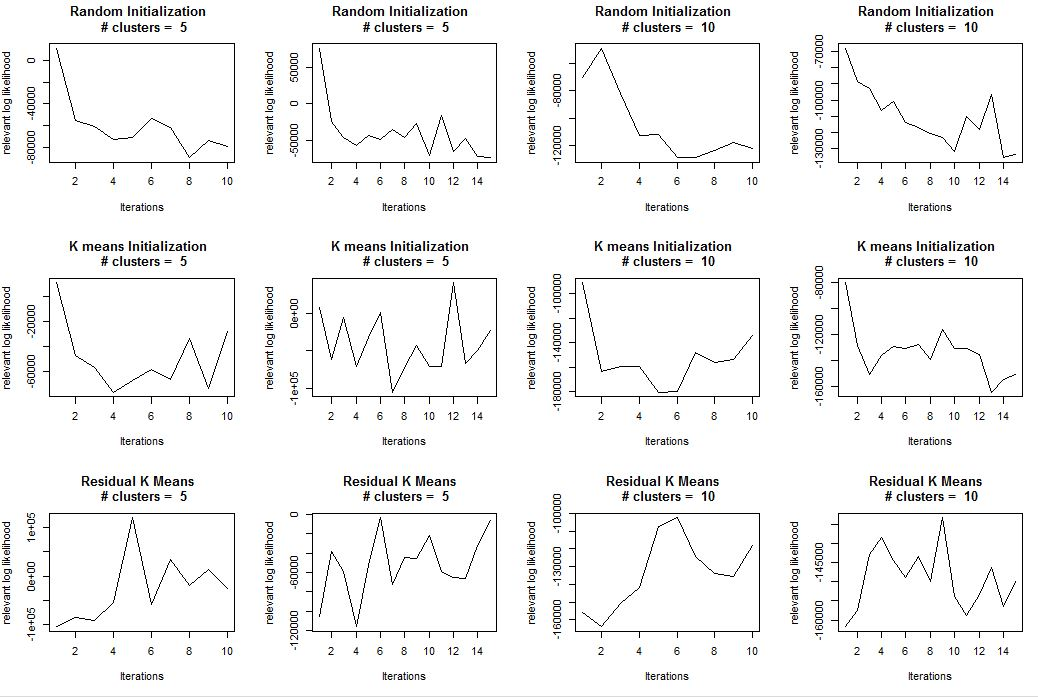
\includegraphics[width=\linewidth]{Images/LikelihoodOfClusters_Iterations}





\subsection{Interpretation of results}
\subsection{Evaluating fit}



\emph{Graphs}

\section{Conclusion}\label{conclusion}







\newpage

\begin{appendix}
\section{Appendix}

\vspace{4mm}\noindent 
The following may be included in an appendix:

\begin{itemize}
\item[] Data 
\item[] Simulation codes
\item[] Certain derivations
\end{itemize}
\end{appendix}
\newpage

\begin{thebibliography}{99}

\bibitem{fisher} Fisher, R. A. (1922). On the mathematical foundations of
theoretical statistics. {\it Philosophical Transactions of the Royal
Society of London} (A) 222: 309-368.

\bibitem{galton} 
Galton, F. (1883). {\it Inquiries into Human Faculty and Its
Development}. London: Macmillan.

\end{thebibliography}
\end{document}
